\documentclass{beamer}
% theme
\usetheme{Berlin}

\usepackage{graphicx}
\usepackage{hyperref}
\usepackage{listings}

\DeclareGraphicsExtensions{.png}

\title{Learning Python}
\author{Erik Edrosa}
\institute [PLUG]{Panther Linux User Group}
\date{} % turns off date

\lstset{language=Python}

\begin{document}
\frame{\maketitle}
\begin{frame}
  \centerline{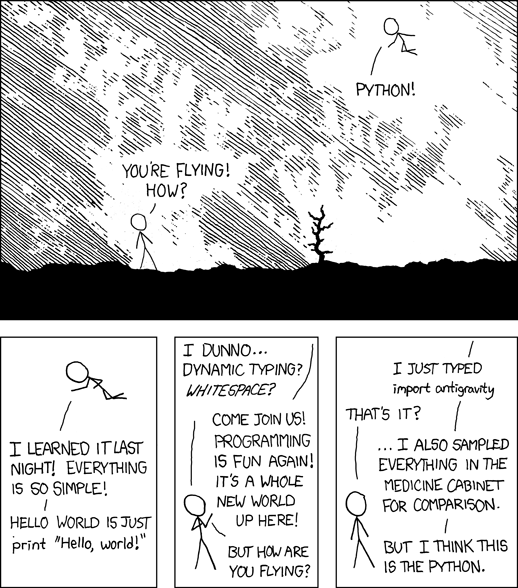
\includegraphics[keepaspectration=true, width=0.5 \textwidth]{python}}
  \centerline{source: \url{http://xkcd.com/353/}}
\end{frame}
\begin{frame}
  \frametitle{What is Python?}
  \begin{quote}
    Python is a programming language that lets you work more quickly and integrate your systems more effectively. You can learn to use Python and see almost immediate gains in productivity and lower maintenance costs
  \end{quote}
  \begin{itemize}
    \item a general purpose high-level programming language
    \item a scripting language
    \item multiple programming paradigms
  \end{itemize}
\end{frame}
\begin{frame}
  \frametitle{How to get Python}
  \begin{itemize}
    \item Linux
      \begin{itemize}
        \item Most distros come with python
        \item type \texttt{python --version} to see which version
        \item if you don't have version 3, use your package manager
          \begin{itemize}
            \item \texttt{sudo apt-get install python3} for Ubuntu
            \item \texttt{sudo pacman -S python} for Arch Linux
          \end{itemize}
      \end{itemize}
    \item Windows
      \begin{itemize}
        \item Download the lastest version from \href{http://python.org}{python.org}
      \end{itemize}
    \item Mac OS X
      \begin{itemize}
        \item Mac OS X comes with python 2.7 pre-installed by apple
        \item Downloaded latest following \href{http://docs.python.org/3.4/using/mac.html}{Using Python on a Mac}
      \end{itemize}
  \end{itemize}
\end{frame}
\begin{frame}
  \frametitle{Python 3 vs. Python 2}
  \begin{itemize}
    \item There is two main versions to download
    \item Important changes were made in Python 3 which breaks compatability with some programs
    \item Support for Python 2 will stop soon
    \item Only develop in Python 2 for maintaining older code which does not support 3
    \item Be sure to check which version you have.
      \begin{itemize}
        \item Some Linux distros have both versions
        \item use \texttt{python --version} to check
        \item Versions might sometimes be named python2 or python3
      \end{itemize}
  \end{itemize}
\end{frame}
\begin{frame}
  \frametitle{Let's get coding}
  \begin{itemize}
    \item The \texttt{python} command is the python interpreter
      \begin{itemize}
        \item Typing \texttt{python} alone runs an interactive interpreter
        \item Typing \texttt{python fileName.py} runs the code in the file
      \end{itemize}
    \item Using the interactive interpreter
      \begin{itemize}
        \item type \texttt{python} or \texttt{python3}
        \item Version info and the symbols \texttt{>>>} will print
        \item \texttt{>>>} is the python prompt
        \item type in \texttt{print("Hello World")}
        \item press enter
        \item \texttt{Hello World} should be printed
        \item type \texttt{exit()} to exit interactive mode
      \end{itemize}
  \end{itemize}
\end{frame}
\begin{frame}
  \frametitle{Basics of Python programming}
  \begin{itemize}
    \item Identation of code is important
      \begin{itemize}
        \item use a tab or two spaces to change the semantics
        \item statments must be on new lines, no semicolons
        \item used to enforce code to be more readable
      \end{itemize}
    \item Python has dynamic typing
      \begin{itemize}
        \item No need to declare the types of variables and arguments
      \end{itemize}
    \item No main function or method
      \begin{itemize}
        \item Python code can run without being in the scope of a function
        \item Main function can be simulated using
          \lstinputlisting[basicstlye=\scriptsize]{exampleMain.py}
      \end{itemize}
  \end{itemize}
\end{frame}
\begin{frame}
  \frametitle{Basic data types}
  \begin{itemize}
    \item Has all your basics like integers, floats, strings, and boolean
    \item A None value which represents the absence of a value
  \end{itemize}
  \centerline{\lstinputlisting{dataTypes.py}}
\end{frame}
\begin{frame}
  \frametitle{Data Structures}
  \begin{itemize}
    \item Lists
      \begin{itemize}
        \item similar to arrays
        \item not a fixed length
        \item items in the list do not need to be the same type
      \end{itemize}
    \item Tuples
      \begin{itemize}
        \item consists of a number of values
        \item is immutable - can not be changed once created
      \end{itemize}
    \item Dictionaries
      \begin{itemize}
        \item Stores keys and values
        \item known as maps or associative arrays in other languages
      \end{itemize}
  \end{itemize}
\end{frame}
\begin{frame}
  \frametitle{Data Structures}
  \framesubtitle{examples}
  \centerline{\lstinputlisting{dataStructures.py}}
\end{frame}
\begin{frame}
  \frametitle{List Comprehensions}
  \begin{itemize}
    \item a concise way to create lists 
    \item same operation can be done using a for loop but in less lines
    \item can even be nested
  \end{itemize}
  \centerline{\lstinputlisting{listComprehensionsExample.py}}
\end{frame}
\begin{frame}
  \frametitle{Variables}
  \begin{itemize}
    \item Remember, python has dynamic typing
    \item Can assign different data types to the same variable and python won't complain
    \item multivariable assignment from expressions which return multiple values
  \end{itemize}
  \centerline{\lstinputlisting{variableExample.py}}
\end{frame}
\begin{frame}
  \frametitle{Control flow}
  \begin{itemize}
    \item Python has the standard control flow statements like if, if else, while, and for
    \item The condition part does not require parenthesis
    \item \texttt{:} follows the condition
    \item the body of the control flow statement is indented and unindented to resume the regular flow
  \end{itemize}
  \centerline{\lstinputlisting{controlflowExample.py}}
\end{frame}
\begin{frame}
  \frametitle{Functions}
  \begin{itemize}
    \item Functions are similar to other languages
    \item First class objects
      \begin{itemize}
        \item means it can be passed around like a normal value
      \end{itemize}
    \item use the \texttt{def} keyword to define a function
    \item there is also lambda (or anonymous functions)
  \end{itemize}
  \centerline{\lstinputlisting{functionExample.py}}
\end{frame}
\begin{frame}
  \frametitle{Classes}
  \begin{itemize}
    \item Python has object oriented programming
    \item Classes are also first class objects
    \item The body of a class are a series of statements, usually function definitions
    \item \texttt{def \_\_init\_\_} is the constructor function
  \end{itemize}
  \centerline{\lstinputlisting{classExample.py}}
\end{frame}
\begin{frame}
  \frametitle{Resources}
  \begin{itemize}
    \item \url{http://python.org}
    \item \href{http://docs.python.org/3/tutorial/index.html}{Python 3 Tutorial}j
    \item \href{http://www.diveinto.org/python3/}{Dive into Python 3}
    \item \href{https://www.udacity.com/course/cs101}{Udacity CS101 (teaches Computer Science in Python)}
  \end{itemize}
\end{frame}
\begin{frame}
  \frametitle{Thank you}
  \framesubtitle{Questions or comments?}
  \begin{itemize}
    \item Contact me at eedro001@fiu.edu
    \item Visit the club's website \url{http://plug.cs.fiu.edu}
    \item Join our irc channel
      \begin{itemize}
        \item plug.cs.fiu.edu
        \item room \#chat
      \end{itemize}
  \end{itemize}
\end{frame}
\end{document}
